
\section{Réseaux de Neurones à Convolution (CNN):}
\begin{center}
	\begin{minipage}{0.4\textwidth}
		\begin{flushleft}
			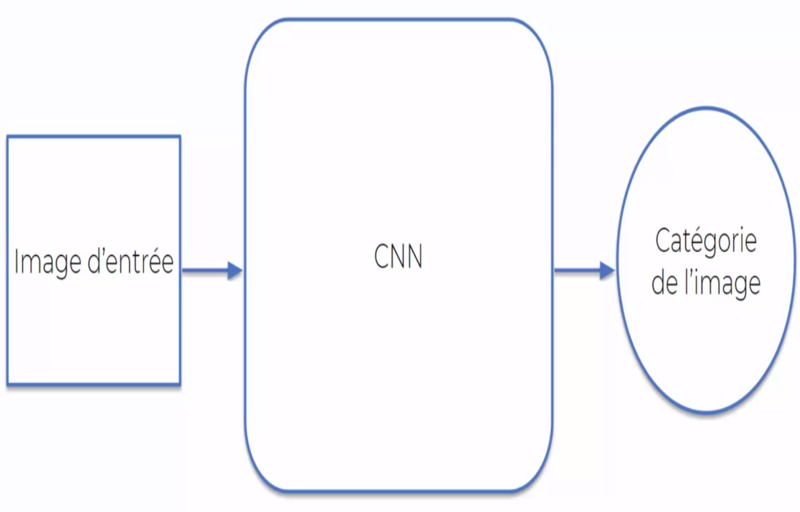
\includegraphics[scale=0.1]{img8.png}
		\end{flushleft}
	\end{minipage}
	\begin{minipage}{0.4\textwidth}
		\begin{flushright}
			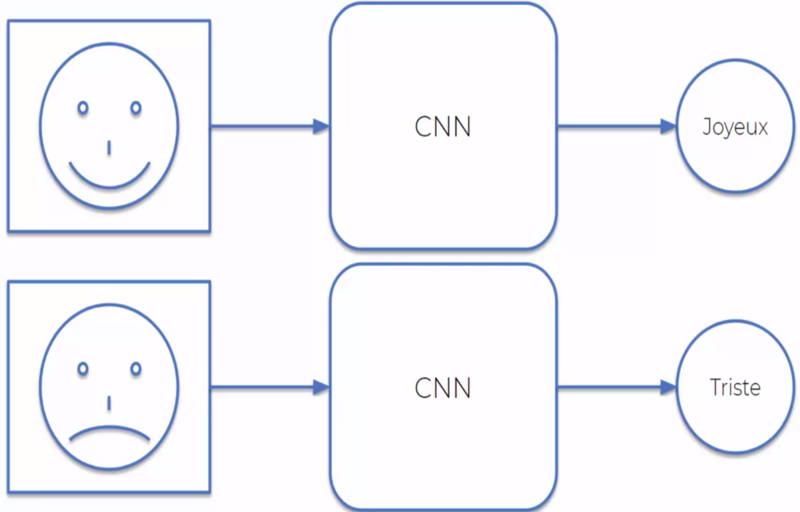
\includegraphics[scale=0.1]{img9.png}  
		\end{flushright}
	\end{minipage}
	\captionof{figure}{https://www.udemy.com/le-deep-learning-de-a-a-z}
\end{center}
\subsection{Définition :}
Les réseaux de neurones convolutifs sont un type particulier de réseaux de neurones multicouches \cite{lecun1995convolutional} et \cite{lecun1998gradient}, inspirer de son ancêtre Le néocognitron \cite{fukushima1980neocognitron}. 
Les réseaux de neurones convolutifs sont conçus pour reconnaître les motifs visuels directement à partir d'images en pixels avec un prétraitement minimal.   
Ils peuvent reconnaître des modèles extrêmement variés (tels que les caractères manuscrits) et robustes aux distorsions et aux transformations géométriques simples. 
\begin{center}
	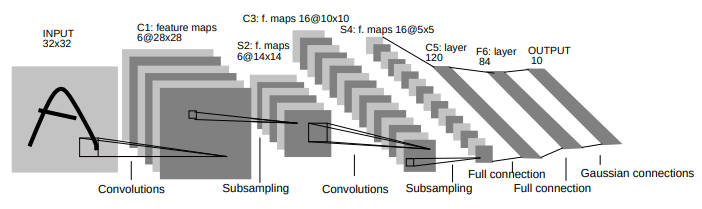
\includegraphics[scale=0.5]{img25.png}
	\captionof{figure}{source \cite{lecun1998gradient}}
\end{center}
\subsection{Les couches de base d'un CNN}
\subsubsection{Opération de Convolution :}
Le filtrage d’une image numérique permet de modifier les valeurs de ces pixels, on peut par exemple chercher à atténuer ces valeurs pour les rend moins nette, à réduire le bruit, ou accentuer ces valeurs pour améliorer la netteté. La dérivation est aussi utilisé pour la détection de contours.\\[1cm]
La formule de convolution :
\begin{center}
	$(f * g)(t) \overset{def}{=} \int_{-\infty}^{+\infty} f(\tau) g(t - \tau) d\tau$
\end{center}
Pour une lecture additionnelle, afin d'avoir une explication mathématique de cette loi je vous propose : 
\cite{wu2017convolutional}.

Pour réaliser l’opération de convolution on considéré :
\begin{itemize}
\item une image X de niveaux de gris dont la valeur au pixel $(i, j)$ est  notée $X_{i,j}$.
\item une matrice convolution (un \textbf{noyau}, \textbf{masque} ou \textbf{Feature Detector}) notée $H$ d’ordre 3 par exemple:
	\begin{center}
		$$\begin{pmatrix}
			h_{0,0} & h_{0,1} & h_{0,2}\\
			h_{1,0} & h_{1,1} & h_{1,2}\\
			h_{2,0} & h_{2,1} & h_{2,2}
		\end{pmatrix}$$
	\end{center}
\end{itemize}
L’image filtrée $Y$ qu’est une carte de caractéristiques (\textbf{Feature Map}) s’obtient en effectuant le produit de convolution entre $X$ et $H$, ce qui donne pour un pixel $(i, j)$ de l’image $Y$ :
\begin{center}
\begin{multline}
Y_{i,j} = h_{0,0}X_{i-1,j-1} + h_{0,1}X_{i-1,j} + h_{0,2}X_{i-1,j+1}\\
     	  + h_{1,0}X_{i,j-1} + h_{1,1}X_{i,j}  + h_{1,2}X_{i,j+1} \\
        	  + h_{2,0}X_{i+1,j-1} + h_{2,1}X_{i+1,j} + h_{2,2}X_{i+1,j+1}
\end{multline}
\end{center}

le pixel $Y_{i,j}$ est obtenu en faisant une combinaison linéaire (moyenne pondérée) du pixel $x_{i,j}$ de l’image initiale et de ses $8$ proches voisins. La relation se généralise aux masques  de convolution $5x5, 7x7$, etc.\\

On voit donc que la relation ne peut s’appliquer sur les bord de l’image donc il faut prévoir un traitement spécial pour eux. On peut par exemple les remplir par la valeur $0$.\\
\begin{center}
	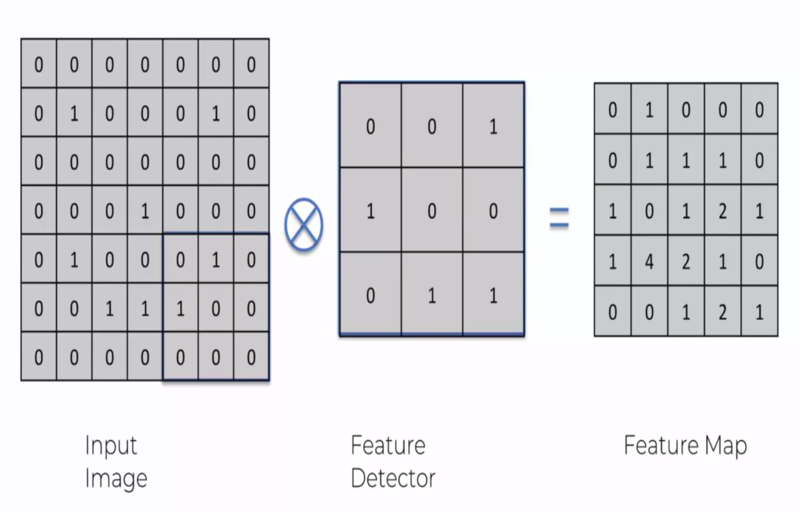
\includegraphics[scale=0.3]{img10.png}
	\captionof{figure}{}
\end{center}

\subsubsection{L’utilité de la convolution : }
\begin{itemize}
\item grâce au cartes des caractéristiques (feature maps) en peut réduire la taille de l’image, donc réduire le temps d’exécution.
\item Les matrice de convolution (feature detector) nous permet de retirer les parties de l’image d’origine qui ne contiennent pas la feature et de repérer les endroit ou la feature apparaît et donc de conserver cette information.
\end{itemize}


Si on réitère ce processus voilà ce qu’on obtient :\\

\begin{center}
	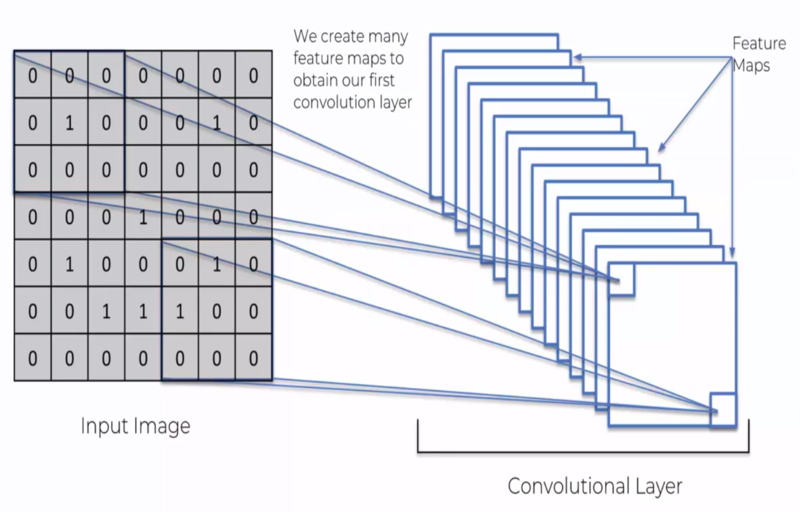
\includegraphics[scale=0.3]{img11.png}
	\captionof{figure}{}
\end{center}

Chaque feature map  correspond à une opération de convolution entre l’image et une  feature detector en particulier ( exemple pour reconnaître un visage par exemple on va avoir un nez, une bouche, un cou, les yeux , etc). Alors ça ce n’est pas forcément nous qui décidons quelles features son importantes mais ça va être le réseau de neurone.

\subsubsection{Couche RELU (Rectifier Linear Unit ou Rectification Linéare):}
Après avoir fait appliquer l’étape de convolution les valeurs de sorties peut être linéaire par rapport à celles en entrée, or dans des images la linéarité n’est pas présente.\\

Pour éviter tous ça, on va utiliser une fonction de redressement , pour que notre modèle soit d’avantage non linéaire ou accentuer la non linéarité \cite{glorot2011deep}.
\begin{eqnarray}
	\phi = \max (x, 0)
\end{eqnarray}

\begin{center}
	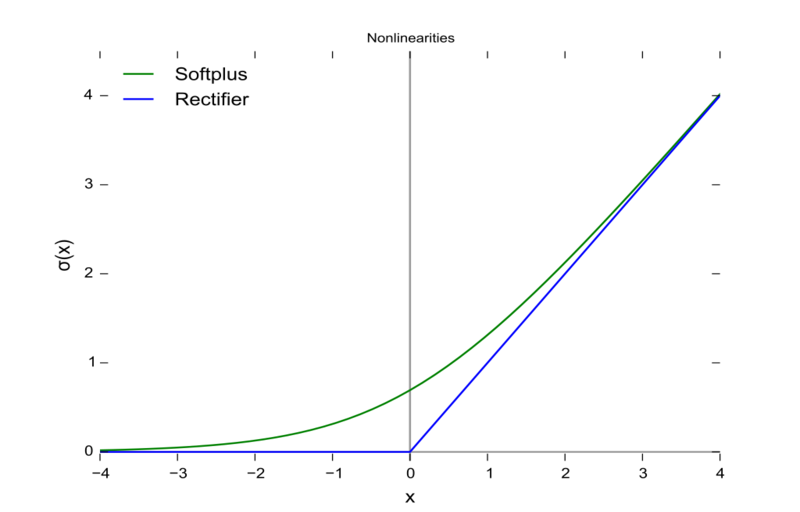
\includegraphics[scale=0.3]{img12.png}
	\captionof{figure}{}
\end{center}

L’utilisation de cette fonction va supprimer une partie des données (les valeurs tous négatives), ce là permet d’accélérer les calculs et d’accentuer beaucoup plus les caractéristiques misent  en évidence par l’étape de convolution. 

\begin{center}
	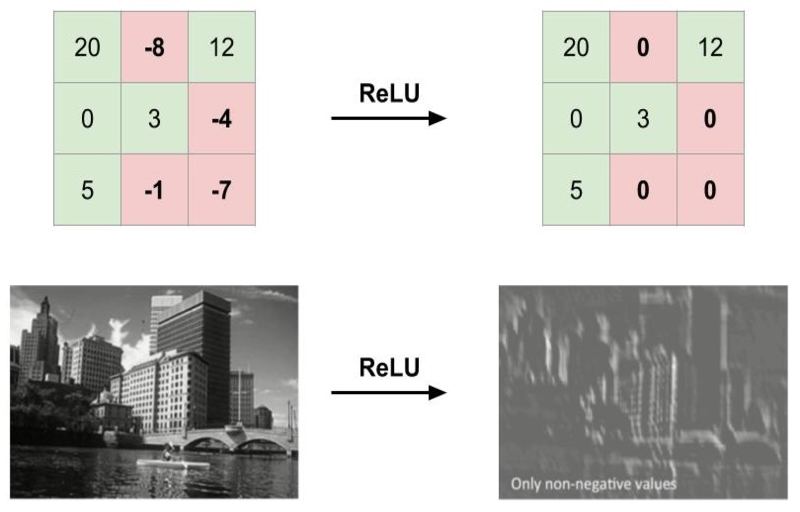
\includegraphics[scale=0.3]{img13.png}
	\captionof{figure}{}
\end{center}
\newpage
\subsubsection{Max Pooling :}
Les réseaux de neurones types CNN ont une propriété qui s’appelle l’invariance spatiale, c’est à dire que pour le réseau rien ne change si les features sont un peut différentes si on zoom, si on les tourne et si on les tord un peut, il doit être suffisamment souple pour pouvoir trouver les features un peut tordues et qu’il puisse identifées que ça correspond exactement à la même chose. Le max pooling est l’opération qui permet de réalise ce là.

\begin{center}
	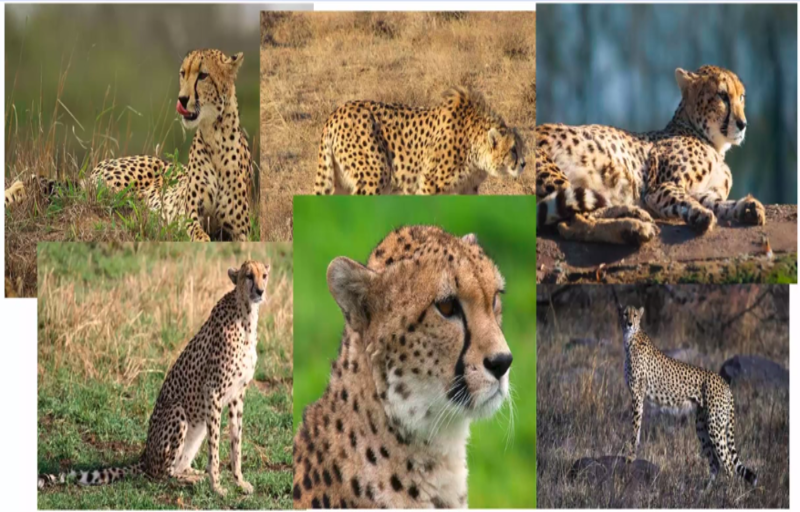
\includegraphics[scale=0.3]{img14.png}
	\captionof{figure}{}
\end{center}

Le max pooling est une opération qui consiste à remplacer une matrice de pixels $(2x2 ou 3x3)$ par une seule valeur, de cette façon l’image diminue en taille et se retrouve lissée.\\

On prend un bloc de $2x2 (3x3)$  et on calcule la valeur qui va remplacé se bloc, ensuite on décale le bloc de $1(2)$ vers la droite, si le bloc sort de l’image  on calcule  avec les pixels qui restent, après on revienne vers la gauche et on décale le bloc de $1(2)$ vers le bas, etc.\\

Pour trouver la valeur qui remplace le bloc $2x2$, il y a différent type de Pooling :

\begin{itemize}
\item Le \textbf{max pooling} : le maximum des valeurs des pixels du bloc, facile et rapide à calculé, c’est le plus utilisé.
\item Le \textbf{mean pooling} : la moyenne des valeurs des pixels du bloc.
\item Le \textbf{sum pooling} : la somme des valeurs des pixels du bloc.
\end{itemize}

\begin{center}
	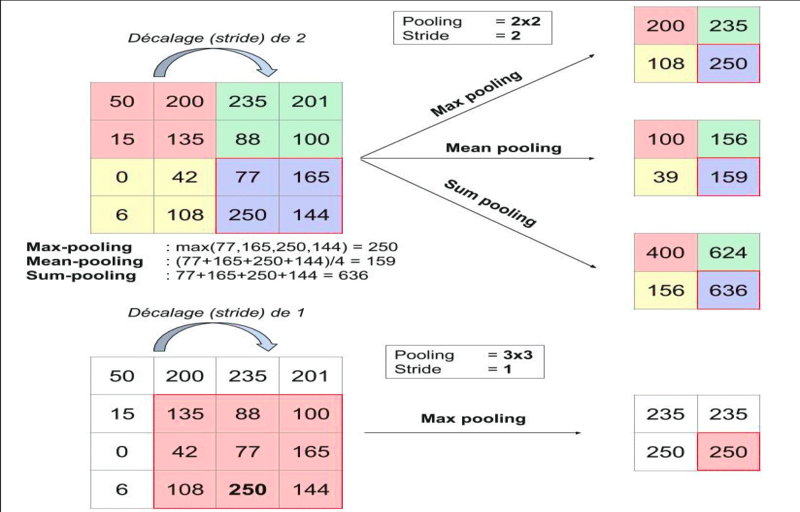
\includegraphics[scale=0.3]{img15.png}
	\captionof{figure}{}
\end{center}

Le max pooling est le plus utilisé car il permet de retenir les caractéristiques les plus importantes et simples. A l’inverse des deux autres, pour une lecture additionnelle \cite{scherer2010evaluation}.

\subsubsection{Flattening : }

L’étape de falttening ça va être d’aplatir complètement les matrices de sorti après l’étape de pooling, en gros on prend les valeurs une par une ligne par ligne et on les aligne dans une colonne.

\begin{center}
	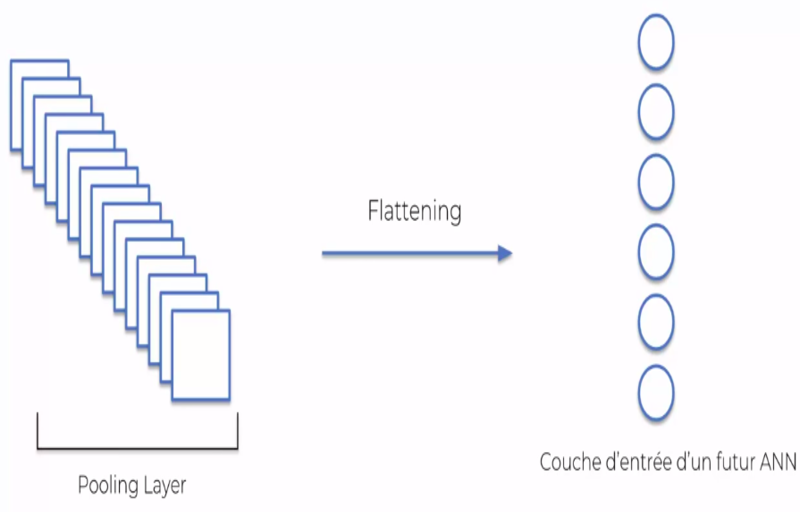
\includegraphics[scale=0.3]{img16.png}
	\captionof{figure}{}
\end{center}

Cette étape va nous permettre de crée un grand vecteur qui sert comme une couche d’entrée d’un futur réseaux de neurones.

\subsubsection{Couche complètement connectée : }

\begin{center}
	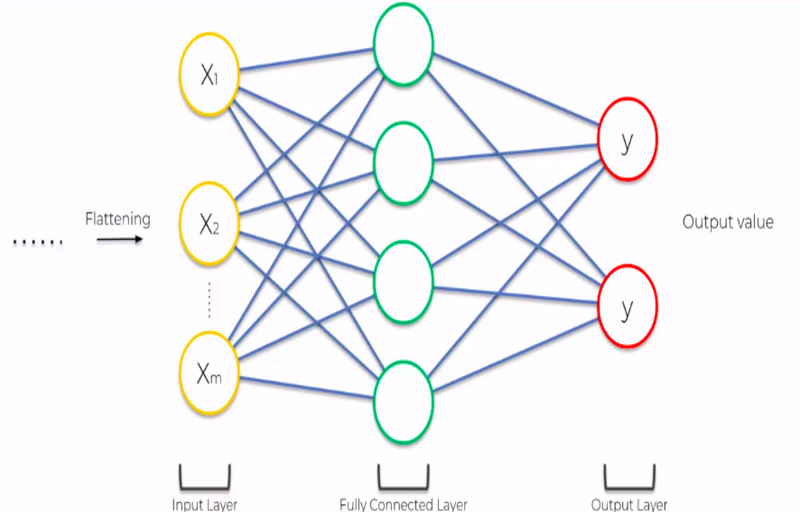
\includegraphics[scale=0.3]{img17.png}
	\captionof{figure}{}
\end{center}

De manière générale cette couche \textit{fully connected} est un perceptron multi-couches.\\
On simplifiant un réseau de neurones artificiels est un réseau qu'est constitue  des neurones:
\begin{itemize}
\item \textbf{Les neurones d'entrés :} envoient leurs valeurs aux neurones de la couche suivante, chaque neurones contient la valeur d'un pixel spécifique.
\item \textbf{Les neurones cachés :} organisés en couches, ils vont envoyer les signaux reçus pondérés par l'importance de leur liaison aux neurones de la couche suivante :
\begin{center}
	$\phi \left( \sum_{i=0}^{m} w_{i}x{i}\right)$ ou $\phi$ est une fonction d'activation.
\end{center} 
\begin{center}
	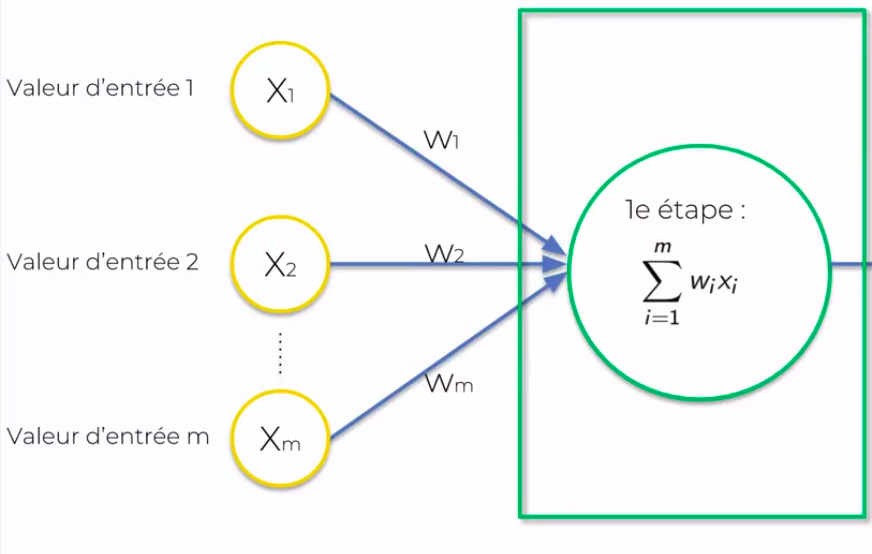
\includegraphics[scale=0.2]{img23.png}
	\captionof{figure}{}
\end{center}
\item \textbf{Les neurones de sortie :} les neurones de cette couche reçoit les signaux pondérés de la coche précédente.\\
Chaque neurones de sortie représente une catégorie, une prédiction spécifique, exemple un neurone qui représente un chien, l'autre un chat, etc...\\
La repense de notre réseau dépend du neurone avec la probabilité la plus forte.
\end{itemize}
Au début de cette couche, l'information va ce propager dans le réseaux de neurones via les synapses, elle va activer des neurones et d'autre non, ce la va crée une premier prédilection.\\
Après le réseau calcule l'erreur avec une fonction coût qu'on aura choisit au préalable.\\
La fonction la plus utilisé est la fonction \textbf{d’entropie croisé}(cross entropie) le but est bien évidement de réduire cette erreur.\\
Ensuite l'erreur est rétro propagée dans le réseau de neurones, et donc on vas ajuster les poids qui sont assignée à chaque synapse avec \textbf{l’algorithme gradient} on va ajusté aussi le feature detector avec un algorithme gradiant adapté au matrice.\\
Tous ce la est afin d'avoir une meilleur prédiction.\\
Ensuite ce procéder  va tourner en boucle pour un bon moment, pour que au final le réseau soit bien entraîné pour donné des bonnes prédictions.\\[1cm]

Au niveau de chaque neurones on applique une certains fonction d'activation $\phi$, parmi ces fonctions d’après \cite{glorot2011deep} :
\begin{itemize}
\item \textbf{La fonction seuil :} 
\begin{center}
	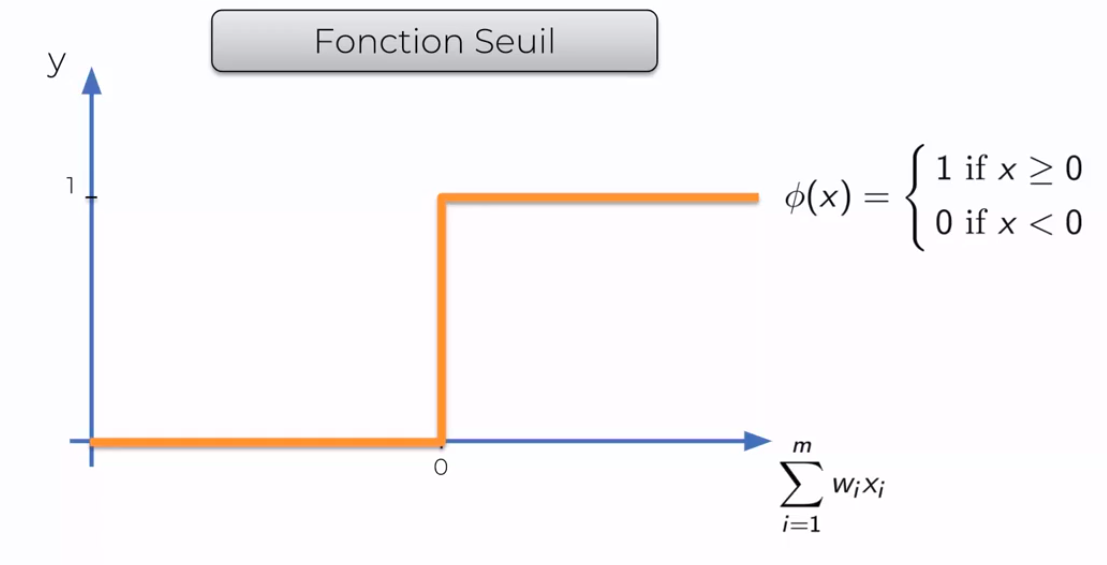
\includegraphics[scale=0.2]{img19.png}
	\captionof{figure}{}
\end{center}
\newpage
\item \textbf{La fonction redresseur :} 
\begin{center}
	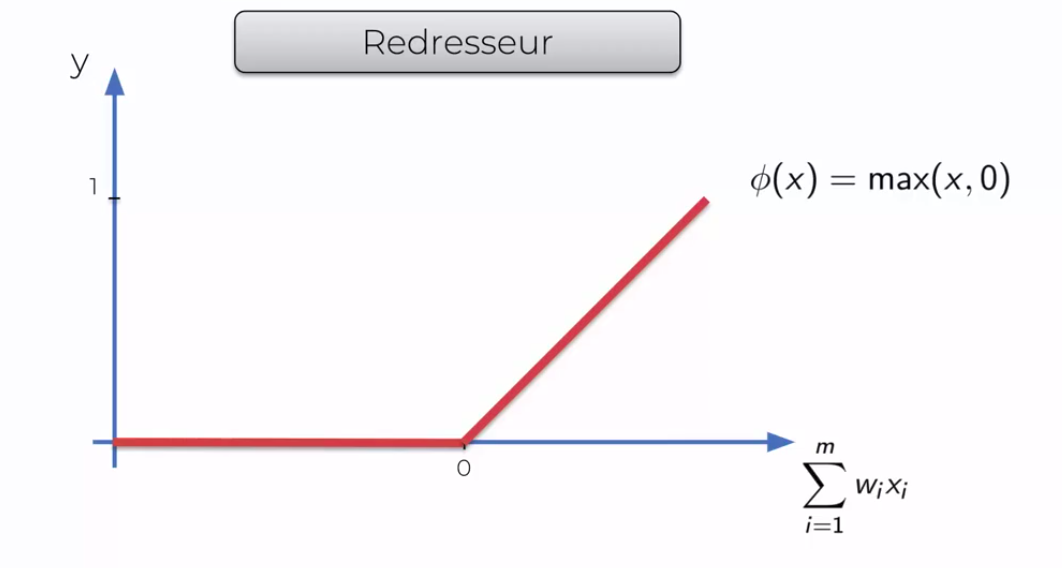
\includegraphics[scale=0.2]{img21.png}
	\captionof{figure}{}
\end{center}
\item \textbf{La fonction sigmoïde :} 
\begin{center}
	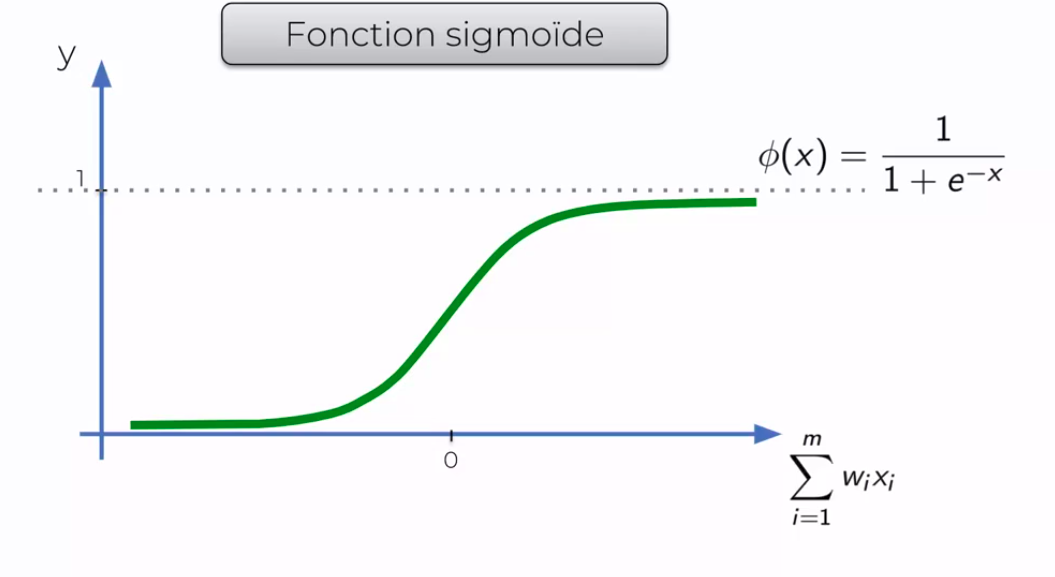
\includegraphics[scale=0.2]{img20.png}
	\captionof{figure}{}
\end{center}
\item \textbf{La fonction hyperbolique (tanh) :} 
\begin{center}
	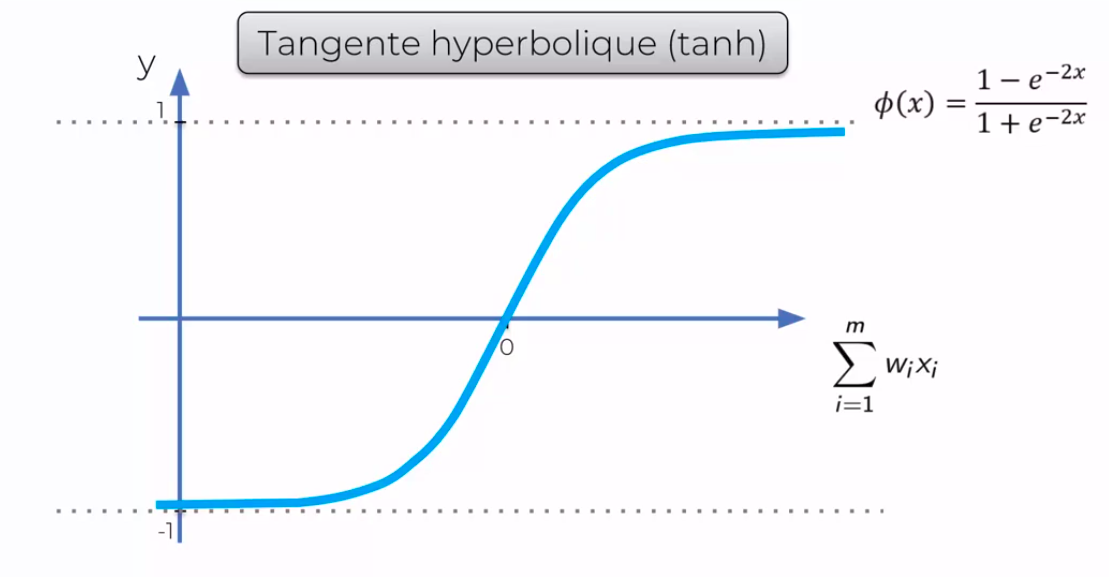
\includegraphics[scale=0.2]{img22.png}
	\captionof{figure}{}
\end{center}
\newpage
\item \textbf{La fonction d’entropie croisé :}\\
Formule originale :
\begin{center}
	$L_{i} = -\log \left( \frac{\exp^{f_{y_{i}}}}{\sum_{j} \exp^{f_{j}}} \right)$
\end{center}
Formule adapter pour le CNN :
\begin{center}
	$H(p, q) = - \sum_{x} p(x)log(q(x))$
\end{center}
Afin d'avoir plus d'explication mathématique \cite{dipietro2016friendly}.
\end{itemize}

\textbf{L’algorithme du gradient :}
\begin{center}
	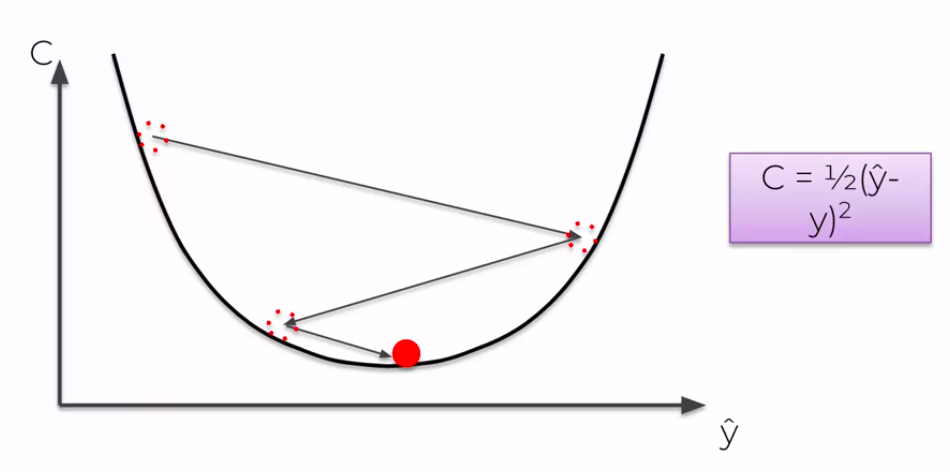
\includegraphics[scale=0.2]{img24.png}
	\captionof{figure}{}
\end{center}
L'algorithme du gradient \cite{lecun1998gradient} désigne un algorithme d'optimisation différentiable.\\
Il est par conséquent destiné à minimiser une fonction réelle différentiable définie sur un espace euclidien (par exemple, ${R} ^{n}$.\\
L'algorithme est itératif et procède donc par améliorations successives. Au point courant, un déplacement est effectué dans la direction opposée au gradient, de manière à faire décroître la fonction.\\
On utilisé pour ce la une fonction de coût :
\begin{center}
	$C = \frac{1}{2} (\hat{y} - y)^{2}$
\end{center}
Ou $y$ : est la vrais valeur, $\hat{y}$ est la valeur du neurone.\\
On modifier les poids des synapses $w_{i}$ de manière a minimisé l'erreur et approcher la bonne solution.\\[1cm]

Les figures de 8 à 21 sont prises du site :\\
\textbf{\href{https://www.udemy.com/le-deep-learning-de-a-a-z/}{https://www.udemy.com/le-deep-learning-de-a-a-z/}}

\newpage
\subsection{Architectures CNN}
A priori on vu l’architectura de base d'un réseau de neurone à convolution, dans la littérature il existe plusieurs type dont l'utilisation et les performances varie en fonction de la tâche qu'il réalise.
parmi ces réseaux de neurones on a :
\begin{itemize}
	\item LeNet (1998) : est un CNN à 7 couches qui classifier des chiffres, développé par LeCun \cite{lecun1998gradient}, il a été utilisé dans plusieurs banque pour reconnaître les nombres manuscrite sur les chèques.
	\begin{center}
		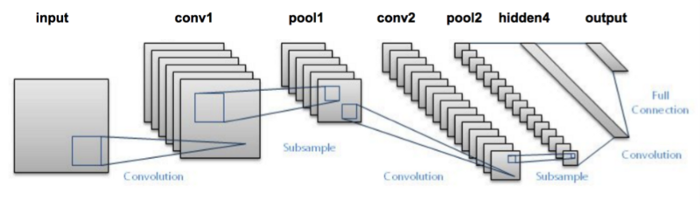
\includegraphics[scale=0.4]{img27.png}
		\captionof{figure}{}
	\end{center}
	\item AlexNet (2012) : c'est l'amléoration de LeNet qui tourne sur un GPU, il a été conçu par le groupe SuperVision, composé d’Alex Krizhevsky, Geoffrey Hinton et Ilya Sutskever.
	\begin{center}
		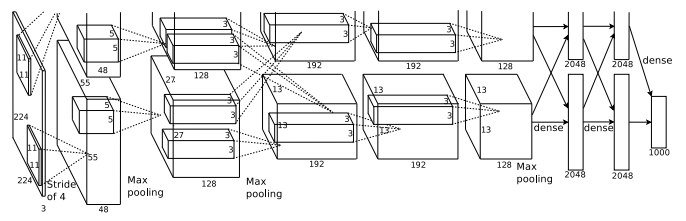
\includegraphics[scale=0.4]{img28.png}
		\captionof{figure}{}
	\end{center}
	\item ZFNet (2013) : est une amélioratiuon de AlexNet.
		\begin{center}
		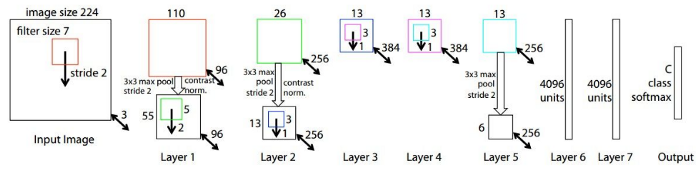
\includegraphics[scale=0.4]{img29.png}
		\captionof{figure}{}
	\end{center}
	\item GoogLeNet/Inception :  C'est l'un des CNN les plus performant, il est utilisé dans la reconnaissance faciale. 
		\begin{center}
		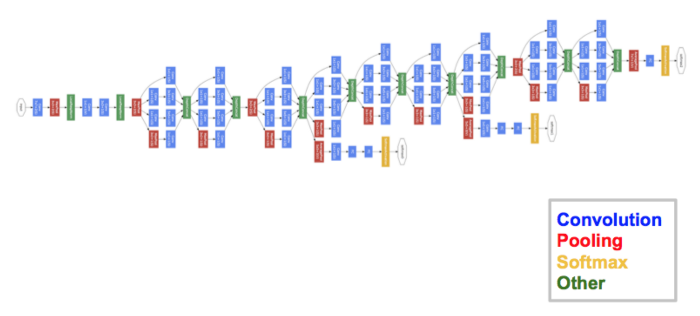
\includegraphics[scale=0.4]{img30.png}
		\captionof{figure}{}
	\end{center}
	\item VGGNet (2014) : Il s'agit du CNN le plus populaire dans l'extraction de fonctionnalités à partir d'images, il est composé de 16 couches et formé sur 4 GPU pendant 2 à 3 semaines, le réseau est crée par Simonyan et Zisserman. 
		\begin{center}
		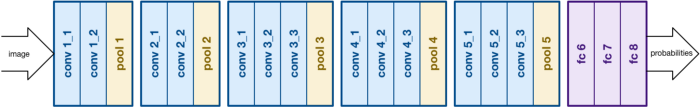
\includegraphics[scale=0.4]{img31.png}
		\captionof{figure}{}
	\end{center}
	\item ResNet (2015) : crée par Kaiming He.
		\begin{center}
		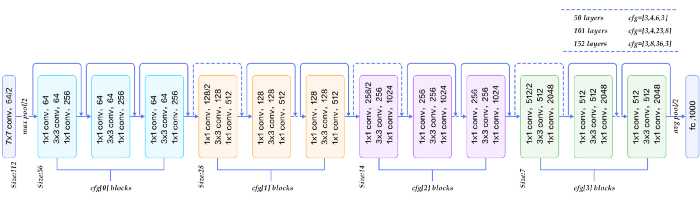
\includegraphics[scale=0.4]{img26.png}
		\captionof{figure}{}
	\end{center}
\end{itemize} 
\newpage
on résumant on a :
\begin{center}
	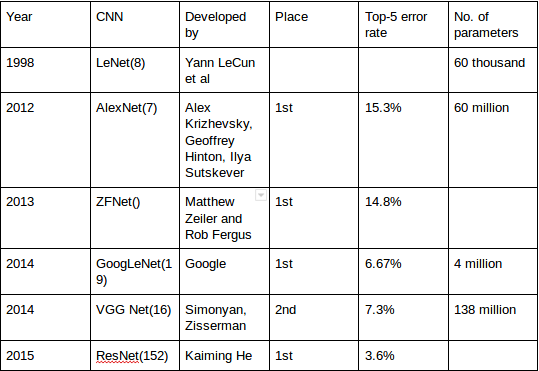
\includegraphics[scale=0.5]{img32.png}
	\captionof{figure}{}
\end{center}
De la figure 22 à la figure 28 sont prélever dans le  site de :\\
\textbf{\href{https://medium.com/@sidereal}{https://medium.com/@sidereal}}